% Presentation for my talk at Saint HighLoad++ 2021
%
% (c) Alexey Naidyonov 2021
% License CC-BY 3.0
%
\documentclass[
  11pt,aspectratio=169,pdf,hyperref={unicode,colorlinks=false}
]{beamer}
\usetheme{shl2021}
\usepackage{pgfpages}
\usepackage{qrcode}

\setbeameroption{hide notes} % Only slides
%\setbeameroption{show only notes} % Only notes
%\setbeameroption{show notes on second screen=right} % Both
\setbeamertemplate{note page}{\pagecolor{yellow!5}\insertnote}

\def\TLA{TLA\textsuperscript{+}}

\title{%
  TLA+/TLC:\\
  формальный метод верификации \\
  конкурентных алгоритмов \\
  для инженеров
}
\author[\href{https://twitter.com/anaidyonov}{@anaidyonov}]{%
  \href{https://twitter.com/anaidyonov}{Алексей Найдёнов}}
\institute[\href{https://itoolabs.com}{ITooLabs}]{%
  \href{https://itoolabs.com}{\resizebox{!}{\baselineskip}{\ITooLabsLogo}}}
\event{\href{https://www.highload.ru/spb/2021}{Saint HightLoad++ 2021}}
\date[20.09.2021]{Sep 20 2021}

\begin{document}

\begin{frame}[plain]\titlepage\end{frame}

\begin{frame}[c]
  \centering\large%
  \vfill%
  \begin{beamercolorbox}{}
    Amazon Web Services \href{http://lamport.azurewebsites.net/tla/formal-methods-amazon.pdf}{%
    \textcolor{blue}{успешно использует \TLA\ Tools}}\textsuperscript{1} с 2011 года\\[2ex]%
    \hfill\begin{minipage}{.95\textwidth}
      \normalsize\itshape%
      ``At AWS, formal methods have been a big success. They have helped us prevent subtle, serious bugs
      from reaching production, bugs that we would not have found via any other technique.''
    \end{minipage}
    \strut\\[2ex]
    \onslide<2>{
    Microsoft использует \TLA\ %
    \href{https://www.microsoft.com/en-us/research/search/?q=TLA\%2B}%
    {\textcolor{blue}{во многих проектах}}\textsuperscript{2},
    включая Azure
    \href{https://docs.microsoft.com/en-us/azure/cosmos-db/consistency-levels}%
    {\textcolor{blue}{CosmosDB}}\textsuperscript{3}%
    \\[2ex]%
    \hfill\begin{minipage}{.95\textwidth}
      \normalsize\itshape%
      ``\TLA\ is not yet a prerequisite for our hiring.
      However, a candidate's knowledge of \TLA\ is given significant weight in
      our evaluation.  To us, it is a great indicator of those who really care
      about quality and correctness.''
    \end{minipage}%
    }
  \end{beamercolorbox}
  \vspace{5ex}%
  \begin{minipage}{\textwidth}
    \fontsize{6.3pt}{10pt}\selectfont\ttfamily\color{black!60}%
    \onslide<1->{%
      1. \href{http://lamport.azurewebsites.net/tla/formal-methods-amazon.pdf}{%
        http://lamport.azurewebsites.net/tla/formal-methods-amazon.pdf}\\
    }%
    \onslide<2->{%
      2. \href{https://www.microsoft.com/en-us/research/search/?q=TLA\%2B}{%
        https://www.microsoft.com/en-us/research/search/?q=TLA\%2B}\\
      3. \href{https://docs.microsoft.com/en-us/azure/cosmos-db/consistency-levels}{%
        https://docs.microsoft.com/en-us/azure/cosmos-db/consistency-levels}\\
    }%
  \end{minipage}
\end{frame}

\begin{frame}[c]
  \centering\large%
  \vfill%
  \begin{beamercolorbox}{}
    MongoDB для
    \href{https://conf.tlapl.us/07_-_TLAConf19_-_William_Schultz_-_Fixing_a_MongoDB_Replication_Protocol_Bug_with_TLA.pdf}{%
      \textcolor{blue}{поиска}}\textsuperscript{1} ошибок в
    \href{https://github.com/will62794/mongo-repl-tla-models}{%
      \textcolor{blue}{протоколе}}\textsuperscript{2}
    репликации
    \\[2ex]%
    \hfill\begin{minipage}{.95\textwidth}
      \normalsize\itshape%
      ``We expect that formally modeling our system upfront could have saved
      100s of hours of engineering time.''
    \end{minipage}
    \strut\\[2ex]
    \onslide<2>{
    CockroachDB для
    \href{https://www.cockroachlabs.com/blog/parallel-commits/}%
    {\textcolor{blue}{спецификации}}\textsuperscript{3} протокола
    \href{https://github.com/cockroachdb/cockroach/tree/master/docs/tla-plus}%
    {\textcolor{blue}{распределенных транзакций}}\textsuperscript{4}%
    \\[2ex]%
    \hfill\begin{minipage}{.95\textwidth}
      \normalsize\itshape%
      ``We found that the process of writing this specification
      gave us more confidence in the Parallel Commit protocol itself
      and in its integration into CockroachDB.''
    \end{minipage}
    }%
  \end{beamercolorbox}
  \vspace{5ex}%
  \begin{minipage}{\textwidth}
    \fontsize{6.3pt}{10pt}\selectfont\ttfamily\color{black!60}%
    \onslide<1->{%
      1. \href{https://conf.tlapl.us/07_-_TLAConf19_-_William_Schultz_-_Fixing_a_MongoDB_Replication_Protocol_Bug_with_TLA.pdf}{%
        conf.tlapl.us/07\_-\_TLAConf19\_-\_William\_Schultz\_-\_Fixing\_a\_MongoDB\_Replication\_Protocol\_Bug\_with\_TLA.pdf}\\
      2. \href{https://github.com/will62794/mongo-repl-tla-models}{%
        github.com/will62794/mongo-repl-tla-models}\\
    }%
    \onslide<2->{%
      3. \href{https://www.cockroachlabs.com/blog/parallel-commits/}{%
        www.cockroachlabs.com/blog/parallel-commits}\\
      4. \href{https://github.com/cockroachdb/cockroach/tree/master/docs/tla-plus}{%
        github.com/cockroachdb/cockroach/tree/master/docs/tla-plus}\\
    }%
  \end{minipage}
\end{frame}

\begin{frame}[c, fragile]
  \begin{center}
    \centering
    \includegraphics[keepaspectratio, height=.7\textheight]{in-and-out.jp2}\\%
    \fontsize{8}{8}\selectfont\color{white!70!black}\copyright The Cartoon Network%
  \end{center}
\end{frame}

% Что такое программа?
\begin{frame}
  \centering\Large\bf{Что такое программа?}
\end{frame}

% Ответ на вопрос
\begin{frame}[c,fragile]
  \begin{columns}
    \begin{column}{.05\textwidth}\end{column}
    \begin{column}{.3\textwidth}
      \begin{code}[fontsize=\large]{go}
        var i = 0
        for i < 3 {
          i = i + 1
        }
      \end{code}
    \end{column}
    \begin{column}{.3\textwidth}
      \centering
      \onslide<2->{\resizebox{!}{.8\textheight}{%
        \begin{tikzpicture}[node distance = 3cm, auto, font=\ttfamily]
          \tikzstyle{decision} = [diamond, draw, text width=4.5em, text badly centered, inner sep=0pt]
          \tikzstyle{block} = [rectangle, draw, text width=5em, text centered, rounded corners, minimum height=4em]
          \tikzstyle{line} = [draw, -latex]
	        \node [block] (init) {i = 0};
	        \node [decision, below of=init] (loop) {i < 3};
	        \node [block, below of=loop] (eval) {i = i + 1};
	        \path [line] (init) -- (loop);
	        \path [line] (loop) -- node [near start] {Yes} (eval);
	        \path [line] (eval.west) |- ([xshift=-2cm]eval.center) -- ([xshift=-2cm]loop.center) -- (loop);
	        \path [line] (loop.east) -- node [near start] {No} ([xshift=2cm]loop.east);
        \end{tikzpicture}
        }
      }
    \end{column}
    \begin{column}{.3\textwidth}
      \centering
      \onslide<3>{\resizebox{!}{.8\textheight}{%
        \begin{tikzpicture}[->,>=stealth',node distance = 1cm, auto]
          \tikzstyle{every state}=[ellipse,font=\ttfamily]
          \node[state] (A)              {i = 0};
          \node[state] (B) [below=of A] {i = 1};
          \node[state] (C) [below=of B] {i = 2};
          \node[state] (D) [below=of C] {i = 3};
          \path (A) edge (B) (B) edge (C) (C) edge (D);
        \end{tikzpicture}
        }
      }
    \end{column}
    \begin{column}{.05\textwidth}\end{column}
  \end{columns}
\end{frame}

% Пример с двумя агентами
\begin{frame}[c,fragile]
  \begin{columns}
  \begin{column}{.2\textwidth}\end{column}
  \begin{column}{.3\textwidth}
    {\Large\bf Process 1}
    \par\vspace{2ex}
    \begin{code}[fontsize=\large]{go}
      a = b + 1
      b = a + 1
    \end{code}
    \par\vspace{5ex}
    {\Large\bf Process 2}
    \par\vspace{2ex}
    \begin{code}[fontsize=\large]{go}
      b = a + 1
      a = b + 1
    \end{code}
  \end{column}
  \begin{column}{.4\textwidth}
  \begin{tikzpicture}[->,>=stealth',node distance=2.5cm and 2cm,semithick,on grid]
    \tikzset{
      state/.style={ellipse,draw,align=left,font=\ttfamily\small},
      edge/.style={->}
    }
    \only<6>{\tikzset{
      state/.prefix style={draw=red}
    }}
    \only<7>{\tikzset{
      edge/.prefix style={draw=blue}
    }}
    \node[state] (A) {a = 0 \\ b = 0};
    \node[left of=A, align=center,red,visible on=<6>] {Состояния\\(states)};
    \node[right of=A, align=center,blue,visible on=<7>] {Пути\\выполнения\\(behaviours)};
    \node[state,visible on={<2-3,6->},label={[visible on={<2-3,6->}]150:p1},align=left] (B) [below left=of A]
      {a = 1\\b = 2};
    \node[state,visible on={<3,6->},label={[visible on={<3,6->}]150:p2},align=left] (C) [below=of B]
      {a = 3\\b = 2};
    \node[state,visible on={<4->},label={[visible on={<4->}]30:p2},align=left] (D) [below right=of A]
      {a = 2\\b = 1};
    \node[state,visible on={<5->},label={[visible on={<5->}]30:p1},align=left] (E) [below=of D]
      {a = 2\\b = 3};
    \path[edge, visible on={<2-3,6->}] (A) edge (B);
    \path[edge, visible on={<3,6->}]   (B) edge (C);
    \path[edge, visible on={<4->}]     (A) edge (D);
    \path[edge, visible on={<5->}]     (D) edge (E);
  \end{tikzpicture}
  \end{column}
  \begin{column}{.2\textwidth}\end{column}
  \end{columns}
\end{frame}

% оценка мощности множества состояний
\begin{frame}[c]
  \Large%
  \begin{gather*}
    (m \cdot n) \frac{(m \cdot n)!}{(n!)^m},
    \intertext{\Large где}
    {\Large \begin{tabular}{>{\(}r<{\)}@{\ --\ }l}
      m & количество процессов \\
      n & длина пути выполнения
    \end{tabular}}
  \end{gather*}
\end{frame}

% пример пространства состояний CAN
\begin{frame}[c]
  \centering
  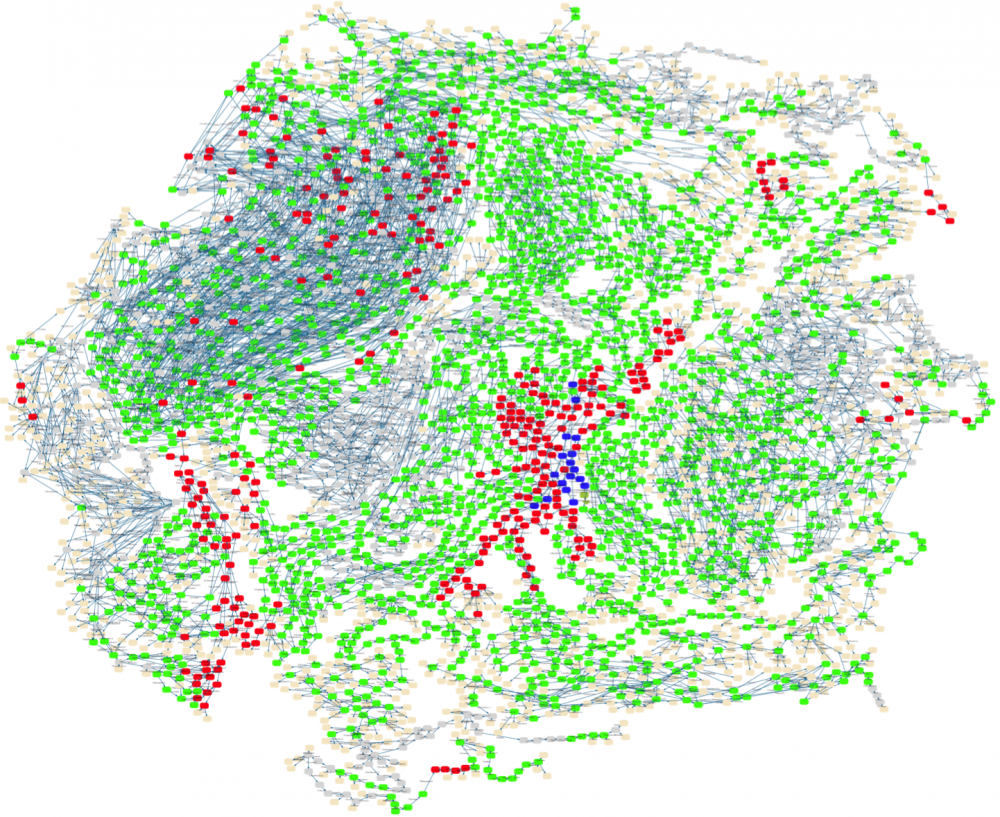
\includegraphics[keepaspectratio, height=.85\textheight]{media/1000px-CANBus_sfdp.png}\\
  {\tiny CAN Bus state space visualization\\[-1\baselineskip]%
  {\color{white!70!black}\url{https://www3.hhu.de/stups/prob/index.php/State_space_visualization_examples}}}
\end{frame}

% штука про отвлечения программиста
\begin{frame}[c]
  \centering
  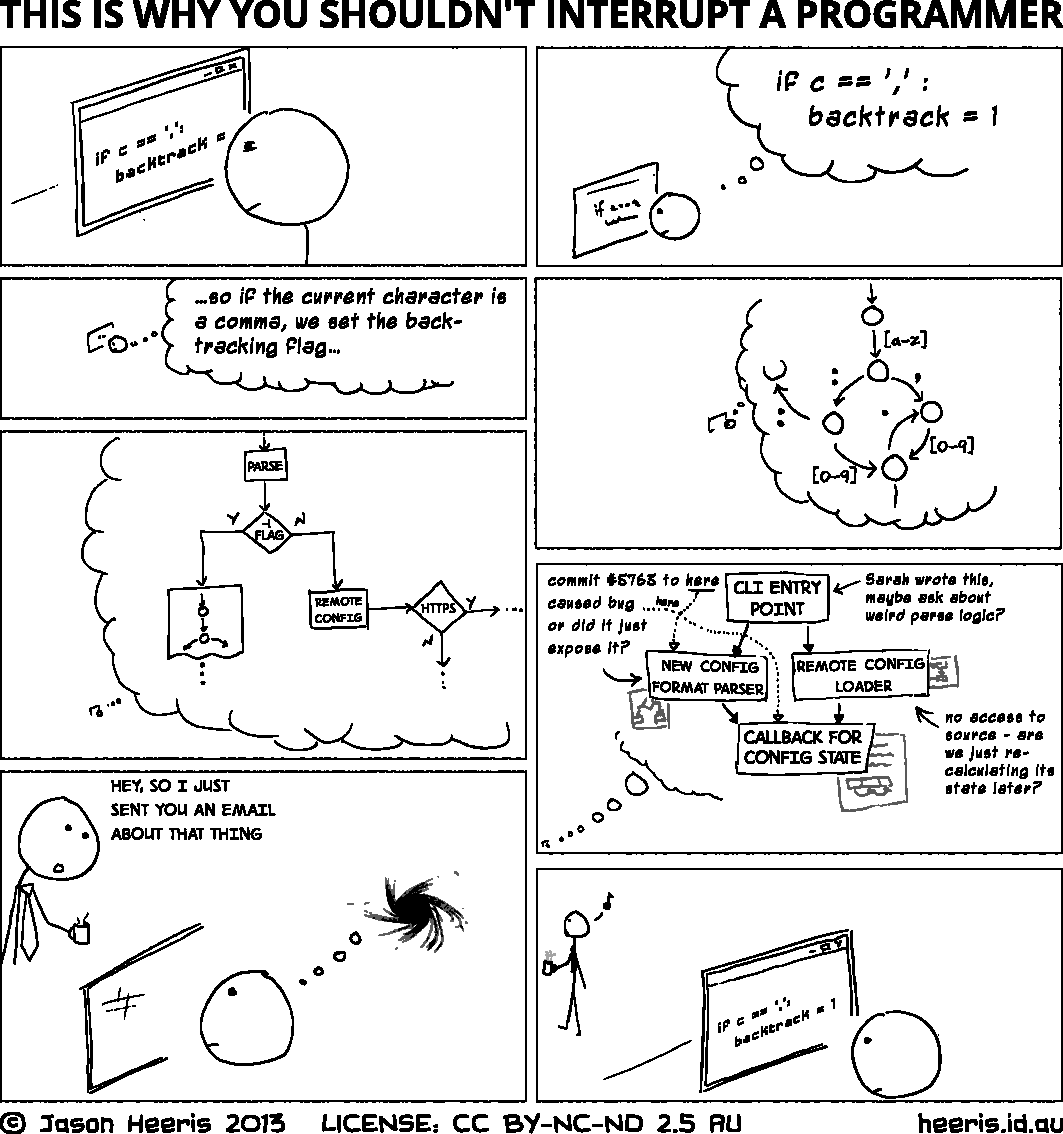
\includegraphics[keepaspectratio, height=.85\textheight]{never-interrupt-programmer.pdf}
\end{frame}

% цитата про распределенные системы
\begin{frame}
  \begin{quote}
    {\Large ``A distributed system is one in which the failure
    of a computer you didn't even know existed can
    render your own computer unusable.''}\\
    \vspace{1ex}
    \hspace*\fill{\small--- Leslie Lamport, May 1987}
  \end{quote}
\end{frame}

% представление Лесли Лэмпорта
\begin{frame}[c]
  \begin{columns}
    \begin{column}{.45\textwidth}
      {\Large\bf
        Лесли Лэмпорт\\
        (\href{https://lamport.azurewebsites.net}{Leslie Lamport})
      }\\
      \vspace{3ex}
      \large
      \vspace{1ex}
      \begin{itemize}
        \item Lamport timestamps
        \item Bakery algorithm
        \item PAXOS
        \item LaTeX
        \item {\bf \TLA}
      \end{itemize}
    \end{column}
    \begin{column}{.5\textwidth}
      \centering
      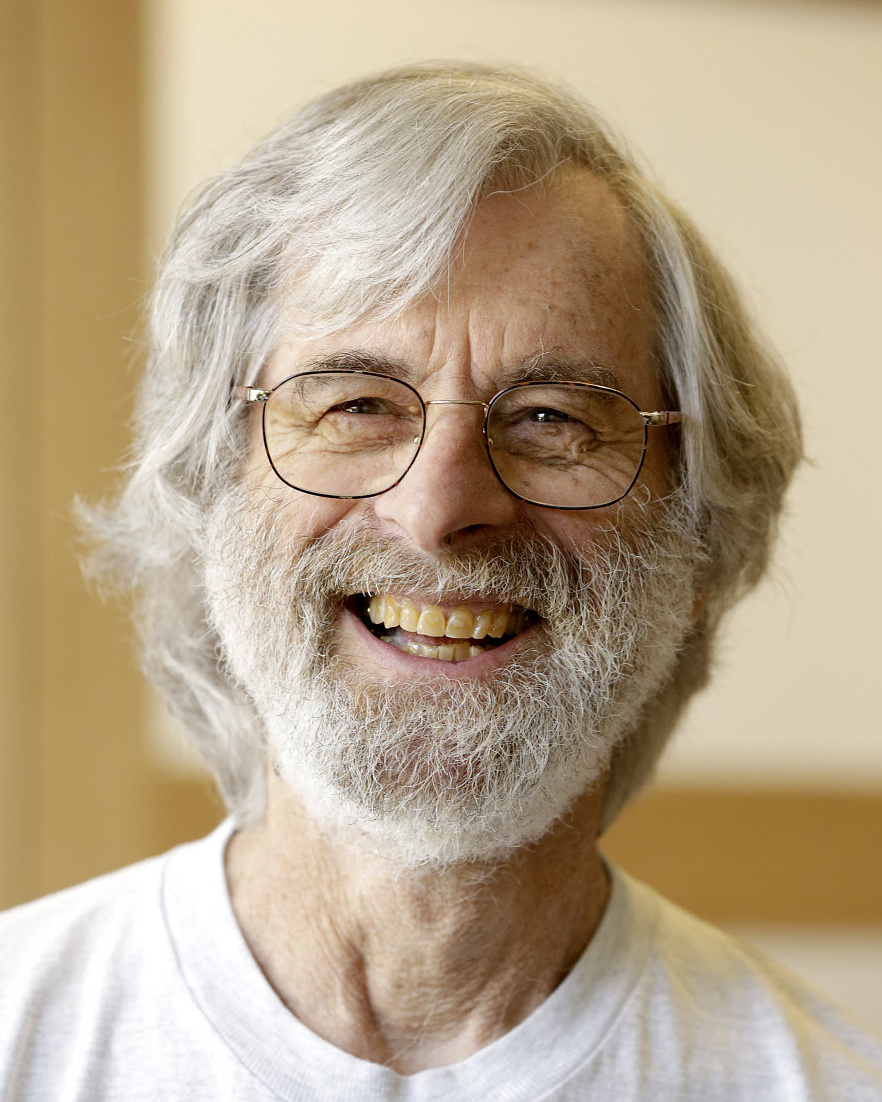
\includegraphics[keepaspectratio, height=.85\textheight]{leslie-lamport.jpeg}
    \end{column}
  \end{columns}
\end{frame}

% TLA+
\begin{frame}[c]
  \centering\Large\bf
  \href{https://lamport.azurewebsites.net/pubs/lamport-actions.pdf}{Temporal Logic of Actions}
\end{frame}

\begin{frame}[c]
  \centering
  \begin{overlayarea}{.7\textwidth}{.8\textheight}
    \centering\large%
    \begin{tabular}{l @{\hspace{3ex}} >{\begin{invisibleenv}<-12>}l<{\end{invisibleenv}} @{\hspace{3ex}} l}
      \multicolumn{3}{c}{\centering\Large\bf\itshape Математическая логика}\pause\\%
      \\%
      \(A \wedge B\)\hspace*{1em}  & \Verb|A/\B| & Conjunction \pause\\%
      \(A \vee B\)                 & \Verb|A\/B| & Disjunction \pause\\%
      \(\neg A\)                   & \Verb|~A|   & Negation    \pause\\%
      \\%
      \multicolumn{3}{c}{\centering\Large\bf\itshape Темпоральная логика}\\%
      \multicolumn{3}{c}{%
        \only<5>{%
          \begin{minipage}{.5\textwidth}%
            \centering\vspace{1.5ex}%
            
\includegraphics[keepaspectratio, height=.35\textheight]{doc-brown.jpg}\\%
            \fontsize{4pt}{1.2}\selectfont\color{white!70!black}\copyright Universal Pictures Amblin Entertainment%
          \end{minipage}%
        }
      }\pause\\%
      \(\Box A\)         & \Verb|[]A|  & Always \pause\\%
      \(\alt<+>{\neg \Box \neg A}{\Diamond A}\) & \Verb|<>A|  & \alt<.>{}{Eventually} \pause\\%
      \(\Diamond\Box A\) \pause & \Verb|<>[]A| & Eventually always \pause\\%
      \(p'\)             \pause & \Verb|p'|    & Next state \pause\\%
    \end{tabular}
  \end{overlayarea}
\end{frame}

% что такое TLA+
\begin{frame}[c]
  \centering
  \begin{overlayarea}{.9\textwidth}{.8\textheight}
    \centering\large
    \begin{tabular}{l @{\hspace{3ex}} l @{\hspace{3ex}} l}
      \multicolumn{3}{c}{\centering\Large\bf\itshape TLA+}\\%
      \\%
      {\tlafont\textsc{true}}  & \Verb|TRUE|          & True \pause\\%
      {\tlafont\textsc{false}} & \Verb|FALSE|         & False \pause\\%
      \(A \triangleq B\)       & \Verb|A == B|        & Define \pause\\%
      \(A = B\)                & \Verb|A = B|         & Equality \pause\\%
      \(A \neq B\)             & \Verb|A /= B|        & Inequality \pause\\%
      \(x \in S\)              & \Verb|x \in S|       & x is in S \pause\\%
      \(x \notin S\)           & \Verb|x \notin S|    & x is not in S \pause\\%
      \(\forall x \in S: P\)   & \Verb|\A x \in S: P| & Universal quantifier \pause\\%
      \(\exists x \in S: P\)   & \Verb|\E x \in S: P| & Existential quantifier
    \end{tabular}
  \end{overlayarea}
\end{frame}

%
% \begin{tabbing}
% ... line \\
% \hl<1>
% line to be highlighted on slide 1 \\
% \end{tabbing}
%
\def\hl<#1>{%
\alt<#1>{\usebeamercolor[fg]{alerted text}}%
        {\usebeamercolor[fg]{normal text}}%
}

%
% disables topsep for tabbing
% einvironment
%
\newenvironment{nstabbing}
{\setlength{\topsep}{0pt}%
  \setlength{\partopsep}{0pt}%
  \tabbing}%
{\endtabbing}

% пример спецификации счетчика
\begin{frame}[c,fragile]
  \begin{columns}
    \begin{column}[c]{.5\textwidth}
    \begin{tlalisting}{00\_Counter}
    \hl<2>
    \begin{tabbing}
      \kw{constants} \= \kill
      \kw{extends}   \> Naturals\\
      [0pt \hl<3>]
      \kw{constants} \> MinValue, MaxValue \\
      [0pt \hl<4>]
      \kw{assume}    \> \( \text{MinValue} < \text{MaxValue} \) \\
      [0pt \hl<5>]
      \kw{variable}  \> counter
    \end{tabbing}
    \begin{nstabbing}
      \\
      [0pt \hl<6>]
      Invariant \= \( \triangleq \text{counter} \in \text{MinValue}\ldotp\ldotp\text{MaxValue} \) \\
      \\
      [0pt \hl<7>]
      Success \> \( \triangleq \Diamond\Box (\text{counter} = \text{MaxValue}) \)
    \end{nstabbing}
    \begin{nstabbing}
      Spec \= \kill \\
      [0pt \hl<8>]
      Init \> \( \triangleq \text{counter} = \text{MinValue} \) \\
      % \pushtabs \\
      \\
      [0pt \hl<9>]
      Next \> \( \triangleq \text{counter}'= \) \= \kw{if} \( \text{counter} < \text{MaxValue} \)
      \+ \+ \\
        \kw{then} counter + 1 \\
        \kw{else} counter \- \- \\
      [0pt \hl<10->]
      Spec \> \( \triangleq \) \= \+ \+ \( \wedge \; \text{Init} \) \\
      [0pt \hl<11->]
        \( \wedge \; \Box[\text{Next}]_\text{counter} \) \\
        [0pt \hl<12>]
        \( \wedge \; \text{WF}_\text{counter}(\text{Next}) \)
    \end{nstabbing}
    \usebeamercolor[fg]{normal text}
  \end{tlalisting}%
  \end{column}
  \begin{column}[c]{.25\textwidth}
    \centering\resizebox{\textwidth}{!}{
\begin{tikzpicture}[>=latex,line join=bevel,]
  \pgfsetlinewidth{1bp}
%%
\begin{scope}
  \pgfsetstrokecolor{black}
  \definecolor{strokecol}{rgb}{1.0,1.0,1.0};
  \pgfsetstrokecolor{strokecol}
  \draw (8.0bp,8.0bp) -- (8.0bp,276.0bp) -- (146.0bp,276.0bp) -- (146.0bp,8.0bp) -- cycle;
\end{scope}
\begin{scope}
  \pgfsetstrokecolor{black}
  \definecolor{strokecol}{rgb}{1.0,1.0,1.0};
  \pgfsetstrokecolor{strokecol}
  \draw (8.0bp,8.0bp) -- (8.0bp,276.0bp) -- (146.0bp,276.0bp) -- (146.0bp,8.0bp) -- cycle;
\end{scope}
\begin{scope}
  \pgfsetstrokecolor{black}
  \definecolor{strokecol}{rgb}{1.0,1.0,1.0};
  \pgfsetstrokecolor{strokecol}
  \draw (8.0bp,8.0bp) -- (8.0bp,276.0bp) -- (146.0bp,276.0bp) -- (146.0bp,8.0bp) -- cycle;
\end{scope}
\begin{scope}
  \pgfsetstrokecolor{black}
  \definecolor{strokecol}{rgb}{1.0,1.0,1.0};
  \pgfsetstrokecolor{strokecol}
  \draw (8.0bp,8.0bp) -- (8.0bp,276.0bp) -- (146.0bp,276.0bp) -- (146.0bp,8.0bp) -- cycle;
\end{scope}
\begin{scope}
  \pgfsetstrokecolor{black}
  \definecolor{strokecol}{rgb}{1.0,1.0,1.0};
  \pgfsetstrokecolor{strokecol}
  \draw (8.0bp,8.0bp) -- (8.0bp,276.0bp) -- (146.0bp,276.0bp) -- (146.0bp,8.0bp) -- cycle;
\end{scope}
  \pgfsetcolor{black}
  % Edge: -107664775997770560 -> -107664775997770560
  \draw [->,dashed] (104.84bp,262.81bp) .. controls (125.69bp,265.31bp) and (145.0bp,261.04bp)  .. (145.0bp,250.0bp) .. controls (145.0bp,240.77bp) and (131.5bp,236.27bp)  .. (104.84bp,237.19bp);
  % Edge: -107664775997770560 -> -8739362515292856379
  \pgfsetcolor{2}
  \draw [->] (68.0bp,231.83bp) .. controls (68.0bp,224.13bp) and (68.0bp,214.97bp)  .. (68.0bp,196.41bp);
  % Edge: -8739362515292856379 -> -8739362515292856379
  \pgfsetcolor{black}
  \draw [->,dashed] (104.84bp,190.81bp) .. controls (125.69bp,193.31bp) and (145.0bp,189.04bp)  .. (145.0bp,178.0bp) .. controls (145.0bp,168.77bp) and (131.5bp,164.27bp)  .. (104.84bp,165.19bp);
  % Edge: -8739362515292856379 -> 1075403382720062154
  \pgfsetcolor{2}
  \draw [->] (68.0bp,159.83bp) .. controls (68.0bp,152.13bp) and (68.0bp,142.97bp)  .. (68.0bp,124.41bp);
  % Edge: 1075403382720062154 -> 1075403382720062154
  \pgfsetcolor{black}
  \draw [->,dashed] (104.84bp,118.81bp) .. controls (125.69bp,121.31bp) and (145.0bp,117.04bp)  .. (145.0bp,106.0bp) .. controls (145.0bp,96.772bp) and (131.5bp,92.275bp)  .. (104.84bp,93.193bp);
  % Edge: 1075403382720062154 -> 8564275020137105871
  \pgfsetcolor{2}
  \draw [->] (68.0bp,87.831bp) .. controls (68.0bp,80.131bp) and (68.0bp,70.974bp)  .. (68.0bp,52.413bp);
  % Edge: 8564275020137105871 -> 8564275020137105871
  \draw [->,dashed] (104.84bp,46.807bp) .. controls (125.69bp,49.308bp) and (145.0bp,45.039bp)  .. (145.0bp,34.0bp) .. controls (145.0bp,24.772bp) and (131.5bp,20.275bp)  .. (104.84bp,21.193bp);
  % Node: -107664775997770560
\begin{scope}
  \definecolor{strokecol}{rgb}{0.0,0.0,0.0};
  \pgfsetstrokecolor{strokecol}
  \definecolor{fillcol}{rgb}{0.83,0.83,0.83};
  \pgfsetfillcolor{fillcol}
  \filldraw [opacity=1] (68.0bp,250.0bp) ellipse (51.99bp and 18.0bp);
  \draw (68.0bp,250.0bp) node {counter = 0};
\end{scope}
  % Node: -8739362515292856379
\begin{scope}
  \definecolor{strokecol}{rgb}{0.0,0.0,0.0};
  \pgfsetstrokecolor{strokecol}
  \draw (68.0bp,178.0bp) ellipse (51.99bp and 18.0bp);
  \draw (68.0bp,178.0bp) node {counter = 1};
\end{scope}
  % Node: 1075403382720062154
\begin{scope}
  \definecolor{strokecol}{rgb}{0.0,0.0,0.0};
  \pgfsetstrokecolor{strokecol}
  \draw (68.0bp,106.0bp) ellipse (51.99bp and 18.0bp);
  \draw (68.0bp,106.0bp) node {counter = 2};
\end{scope}
  % Node: 8564275020137105871
\begin{scope}
  \definecolor{strokecol}{rgb}{0.0,0.0,0.0};
  \pgfsetstrokecolor{strokecol}
  \draw (68.0bp,34.0bp) ellipse (51.99bp and 18.0bp);
  \draw (68.0bp,34.0bp) node {counter = 3};
\end{scope}
%
\end{tikzpicture}

}%
  \end{column}
  \end{columns}
\end{frame}

% что такое TLC
\begin{frame}[c]
  \centering
  {\Large\bf TLC}
  \par\vspace{2ex}
  \Large
  Explicit State Model Checker for \TLA
\end{frame}

% TLA+ Toolbox
\begin{frame}[c, fragile]
  \frametitle{{\href{https://github.com/tlaplus/tlaplus/releases/}{\TLA\ Toolbox} by Simon Zambrovski, et al.}}
  \vskip-8pt
  \begin{tikzpicture}[remember picture, every node/.style={inner sep=0,outer sep=0}]
    \node at (0,0) [anchor=south west]{
      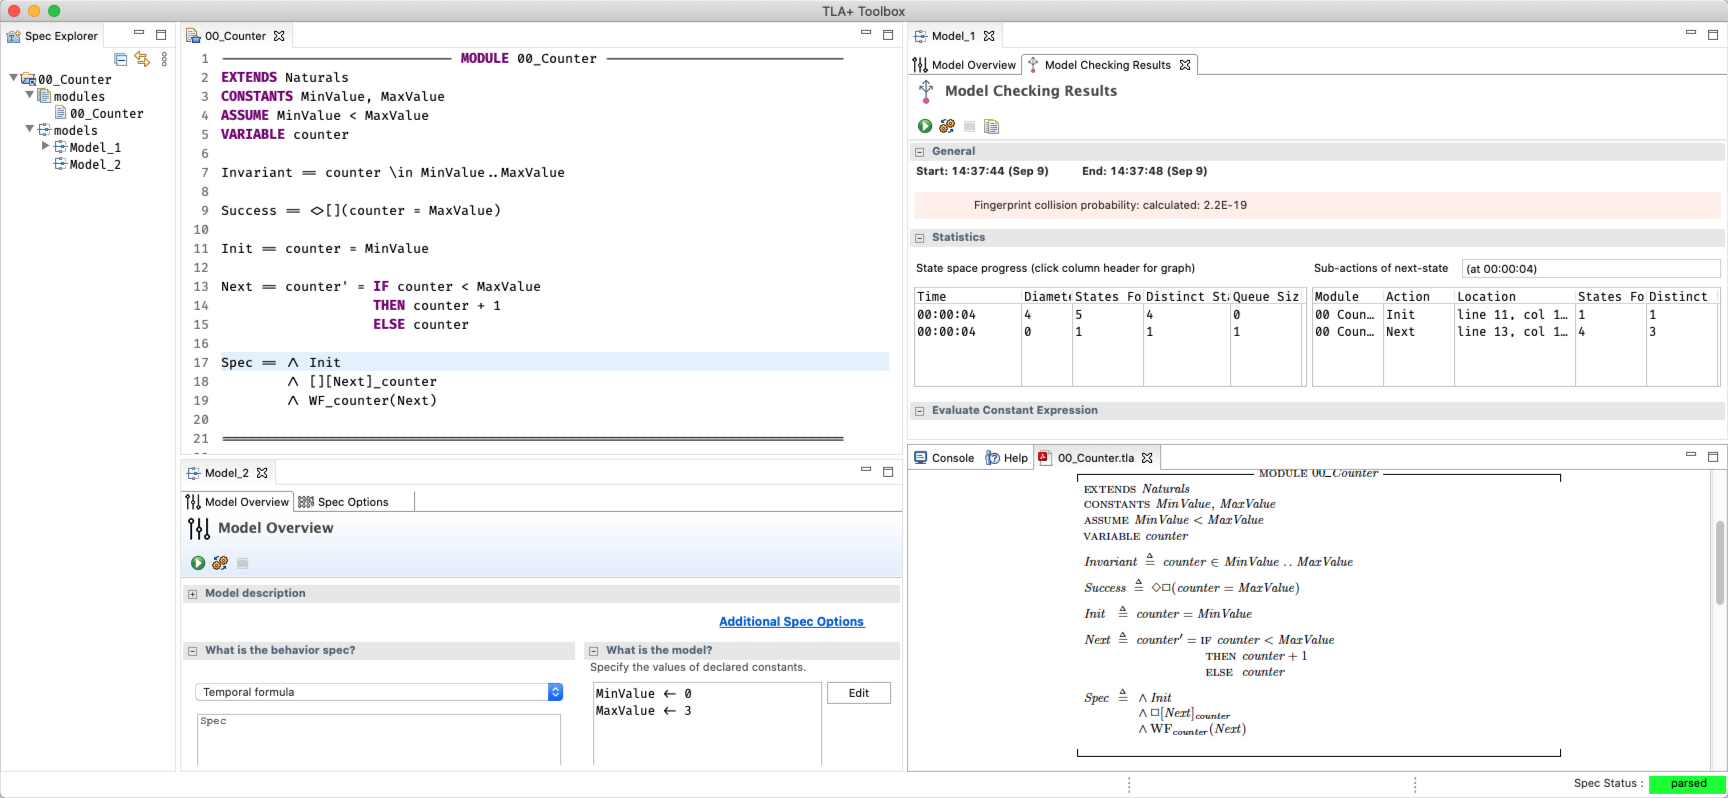
\includegraphics{tla-toolbox-screenshot.png}
    };
    \draw[visible on=<2>,red] (1.51,2.86) rectangle (7.52,6.46);
    \draw[visible on=<3>,red] (1.51,0.22) rectangle (7.52,2.82);
    \draw[visible on=<4>,red] (7.56,2.98) rectangle (14.38,6.46);
  \end{tikzpicture}%
\end{frame}

% Visual Studio Code
\begin{frame}[c, fragile]%
  \frametitle{\href{https://code.visualstudio.com/download}{VS Code}~/~%
  \href{https://marketplace.visualstudio.com/items?itemName=alygin.vscode-tlaplus}{\TLA\ Support by Андрей Лыгин}%
  ~{\href{https://github.com/alygin}{@alygin}}%
  }%
  \vskip-8pt
  \begin{tikzpicture}[every node/.style={inner sep=0,outer sep=0}]
    \node at (0,0) [anchor=south west]{
      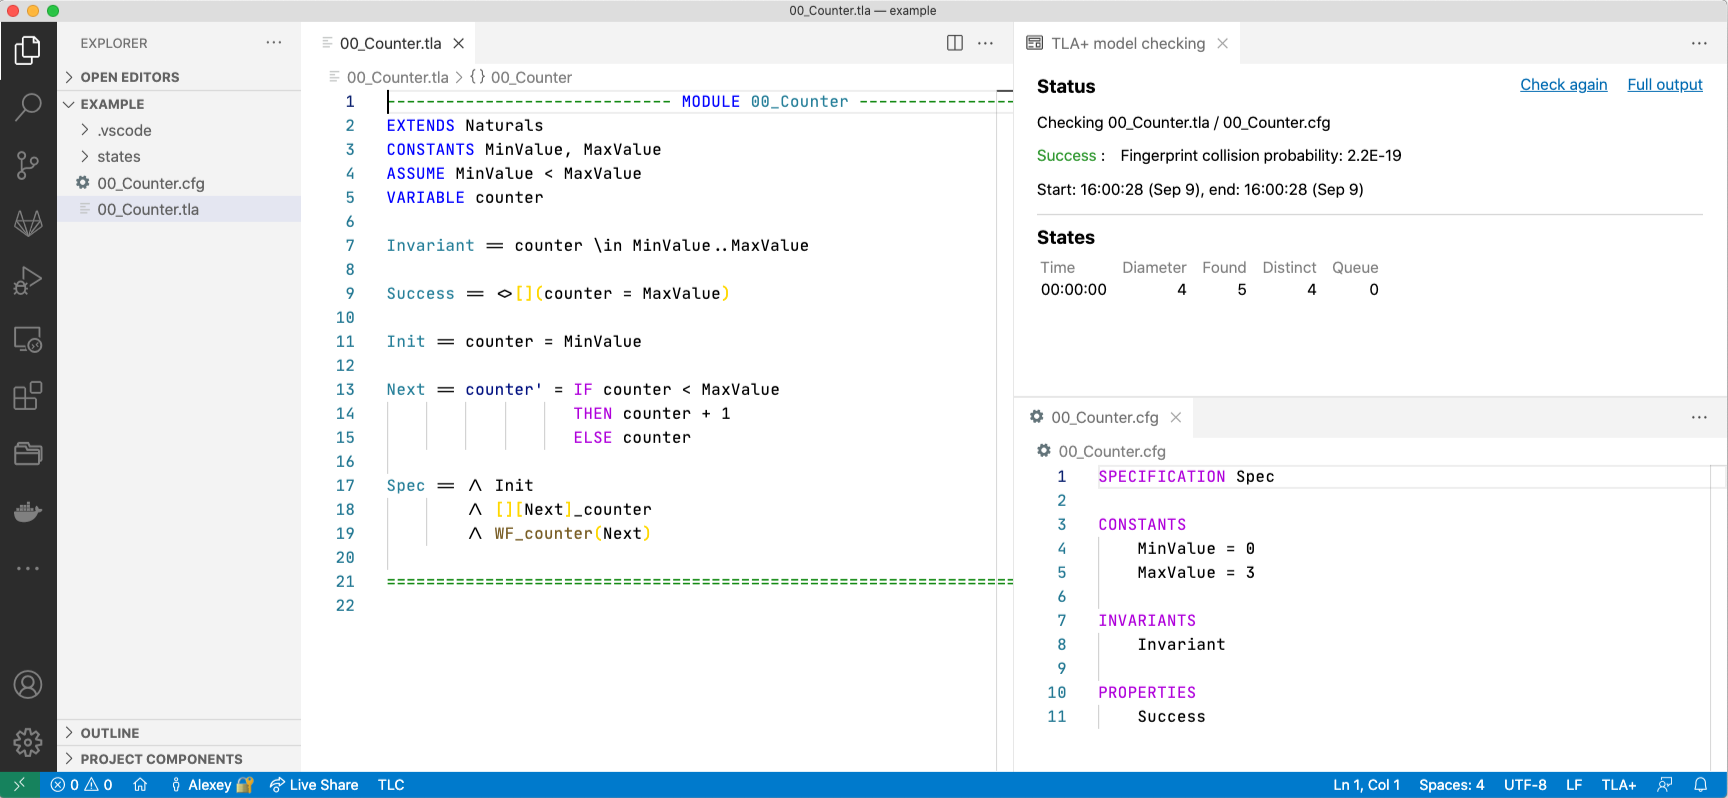
\includegraphics[width=\textwidth, height=.75\textheight]{tla-vscode-screenshot.png}
    };
    \draw[visible on=<2>,red] (2.50,0.225) rectangle (8.45,6.46);
    \draw[visible on=<3>,red] (8.45,0.225) rectangle (14.38,3.38);
    \draw[visible on=<4>,red] (8.45,3.390) rectangle (14.38,6.46);
  \end{tikzpicture}%
\end{frame}

% что такое PlusCal
\begin{frame}[c]
  \centering
  {\Large\bf PlusCal}
\end{frame}

% PlusCal
\begin{frame}[t,fragile]
  \frametitle{PlusCal}
  \framesubtitle<1>{\strut{}~}%
  \framesubtitle<2>{Алгоритм}%
  \framesubtitle<3>{Переменные}%
  \framesubtitle<4>{Определения \TLA}%
  \framesubtitle<5>{Процессы}%
  \framesubtitle<6>{Метки}%
  \only<2>{\setminted{highlightlines={4,26}}}%
  \only<3>{\setminted{highlightlines={6-8}}}%
  \only<4>{\setminted{highlightlines={10-12}}}%
  \only<5>{\setminted{highlightlines={14-18,20-24}}}%
  \only<6>{\setminted{highlightlines={15,21}}}%
  \begin{minipage}{\textwidth}
    \begin{columns}[T]
      \begin{column}{.45\textwidth}
        \inputtla[fontsize=\small,firstline=4,lastline=12]{01_PCDemo.tla}
      \end{column}
      \begin{column}{.45\textwidth}
        \inputtla[fontsize=\small,firstline=14,lastline=26]{01_PCDemo.tla}
      \end{column}
    \end{columns}
  \end{minipage}
\end{frame}

% PlusCal
\begin{frame}[t,fragile]
  \frametitle{PlusCal}
  \framesubtitle{Трансляция}
  \only<+>{\setminted{highlightlines={28,34}}}%
  \only<+>{\setminted{highlightlines={36}}}%
  \only<+>{\setminted{highlightlines={41,42}}}%
  \inputtla[fontsize=\small,firstline=27,lastline=31]{01_PCDemo.tla}%
  \inputtla[fontsize=\small,firstline=34,lastline=42]{01_PCDemo.tla}%
\end{frame}

\begin{frame}[t,fragile]
  \frametitle{PlusCal}
  \framesubtitle{Трансляция}
  \only<+>{\setminted{highlightlines={44,51}}}%
  \only<+>{\setminted{highlightlines={47,54}}}%
  \inputtla[fontsize=\small,firstline=44,lastline=56]{01_PCDemo.tla}%
\end{frame}

\begin{frame}[t,fragile]
  \frametitle{PlusCal}
  \framesubtitle{Трансляция}
  \only<+>{\setminted{highlightlines={59,60,69}}}%
  \only<+>{\setminted{highlightlines={62,63}}}%
  \only<+>{\setminted{highlightlines={65-67}}}%
  \inputtla[fontsize=\small,firstline=58,lastline=69]{01_PCDemo.tla}%
\end{frame}

% Демо -- два агента
\begin{frame}[c]
  \centering{\Large\bf ДЕМО}\\[2ex]%
  {\normalsize\ttfamily\textcolor{black!80}{01\_PCDemo.tla}}
\end{frame}

% TLA+ Toolbox CLI
\definecolor{shellbgcolor}{rgb}{1,0.99,0.96}
\begin{frame}[c,fragile]
  \frametitle{\TLA\ Toolbox CLI}
  \begin{tcolorbox}[colback=shellbgcolor,boxrule=.25pt]%
    \scriptsize%
    \begin{Verbatim}[commandchars=\\\{\}]
\textcolor[HTML]{D78600}{growler@macbook}:\textcolor{green!90!black}{$} tlc -dump dot,colorized 01_PCDemo.dot 01_PCDemo.tla
\textcolor{black!50}{Computing initial states...}
\textcolor{black!50}{Finished computing initial states: 1 distinct state generated.}
\textcolor{black!50}{Checking 2 branches of temporal properties for the complete state space}
\textcolor{black!50}{  with 10 total distinct states}
\textcolor{black!50}{Finished checking temporal properties}
\textcolor{black!50}{Model checking completed. No error has been found.}
\textcolor{black!50}{  Estimates of the probability that TLC did not check all reachable states}
\textcolor{black!50}{  because two distinct states had the same fingerprint:}
\textcolor{black!50}{  calculated (optimistic):  val = 5.4E-19}
\textcolor{black!50}{7 states generated, 5 distinct states found, 0 states left on queue.}
\textcolor[HTML]{D78600}{growler@macbook}:\textcolor{green!90!black}{$} dot -Tsvg 01_PCDemo.dot -o 01_PCDemo.svg
\textcolor[HTML]{D78600}{growler@macbook}:\textcolor{green!90!black}{$}
    \end{Verbatim}
  \end{tcolorbox}
\end{frame}

% TLA+ ToolBox -- States diagram
\begin{frame}[c]
  \begin{center}
    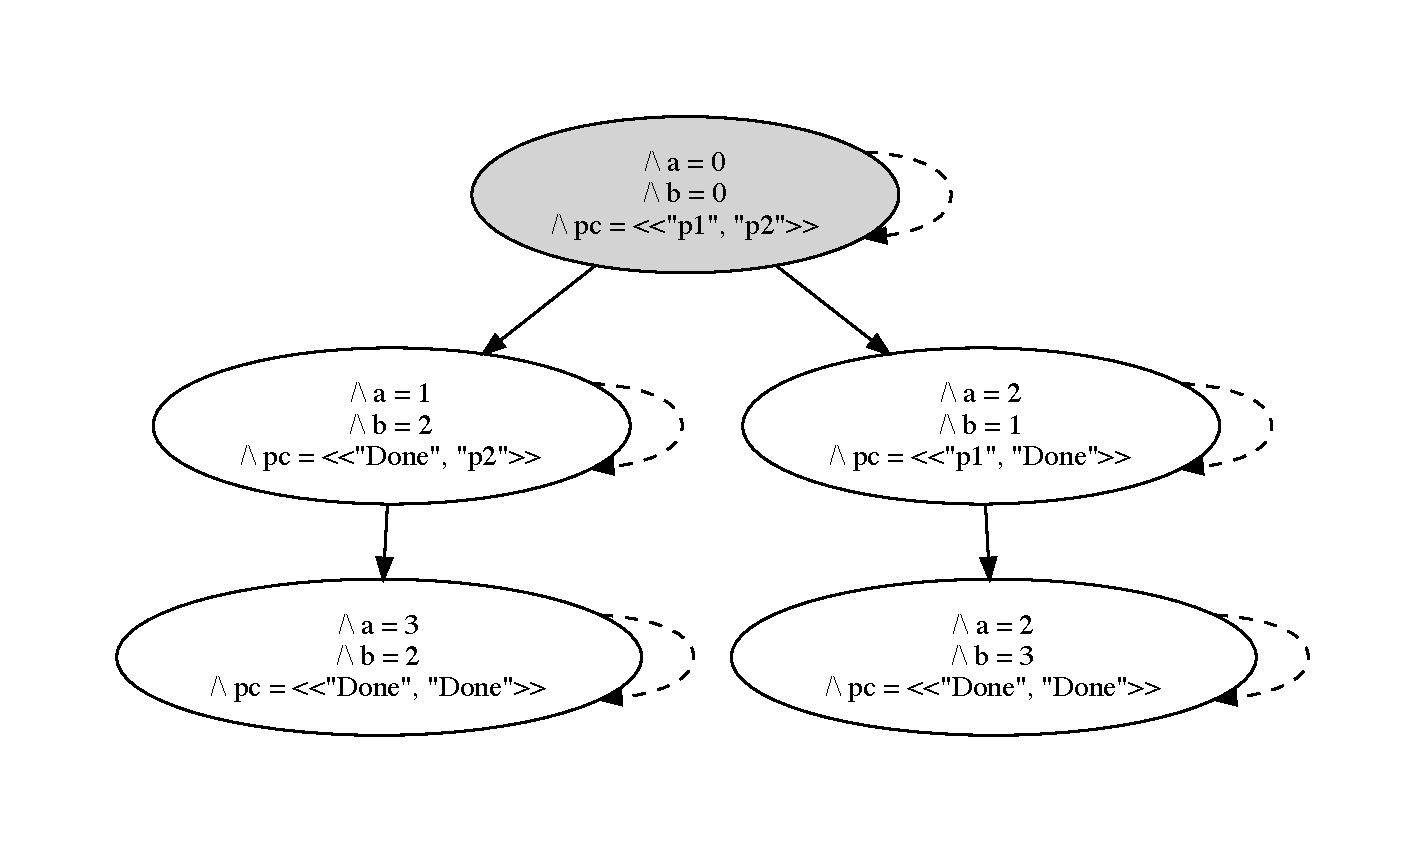
\includegraphics[keepaspectratio, height=.9\textheight]{01_PCDemo.pdf}%
  \end{center}
\end{frame}

% PlusCal -- атомарность
\begin{frame}[c,fragile]
  \frametitle{PlusCal}
  \framesubtitle{Атомарность}
  \setminted{highlightlines={18,19,24,25}}%
  \begin{columns}[T]
    \begin{column}{.45\textwidth}
      \inputcode[fontsize=\small,firstline=4,lastline=14]{tla}{02_PCDemo.tla}
    \end{column}
    \begin{column}{.45\textwidth}
      \inputcode[fontsize=\small,firstline=16,lastline=28]{tla}{02_PCDemo.tla}
    \end{column}
  \end{columns}
\end{frame}

\newcommand{\vhl}[2]{\alt<#1>{\bf\ttfamily\textcolor{red!90!black}{#2}}{#2}}
% Демо -- гонки
\begin{frame}[c,fragile]
  \begin{tcolorbox}[colback=shellbgcolor,boxrule=.25pt]%
  \centering\tiny%
  \begin{Verbatim}[commandchars=!\{\}]
    !vhl{2-}{Error: Temporal properties were violated.}

    !vhl{3-}{Error: The following behavior constitutes a counter-example:}

    State 1: <Initial predicate>
    /\ a = 0
    /\ b = 0
    /\ pc = <<"p1_1", "p2_1">>

    State 2: <p1_1 line 48, col 9 to line 51, col 17 of module 02_PCDemo>
    /\ a = 1
    /\ b = 0
    /\ pc = <<"p1_2", "p2_1">>

    State 3: <p2_1 line 60, col 9 to line 63, col 17 of module 02_PCDemo>
    /\ a = 1
    /\ b = 2
    /\ pc = <<"p1_2", "p2_2">>

    State 4: <p2_2 line 65, col 9 to line 68, col 17 of module 02_PCDemo>
    /\ a = 3
    /\ b = 2
    /\ pc = <<"p1_2", "Done">>

    !vhl{4}{State 5: <p1_2 line 53, col 9 to line 56, col 17 of module 02_PCDemo>}
    !vhl{4}{/\ a = 3}
    !vhl{4}{/\ b = 4}
    /\ pc = <<"Done", "Done">>
  \end{Verbatim}
\end{tcolorbox}
\end{frame}

% Демо -- гонки
\begin{frame}[c]
  \centering\resizebox{\textwidth}{!}{%
  \begin{tikzpicture}
    \node[anchor=south west,inner sep=0] at (0,0) {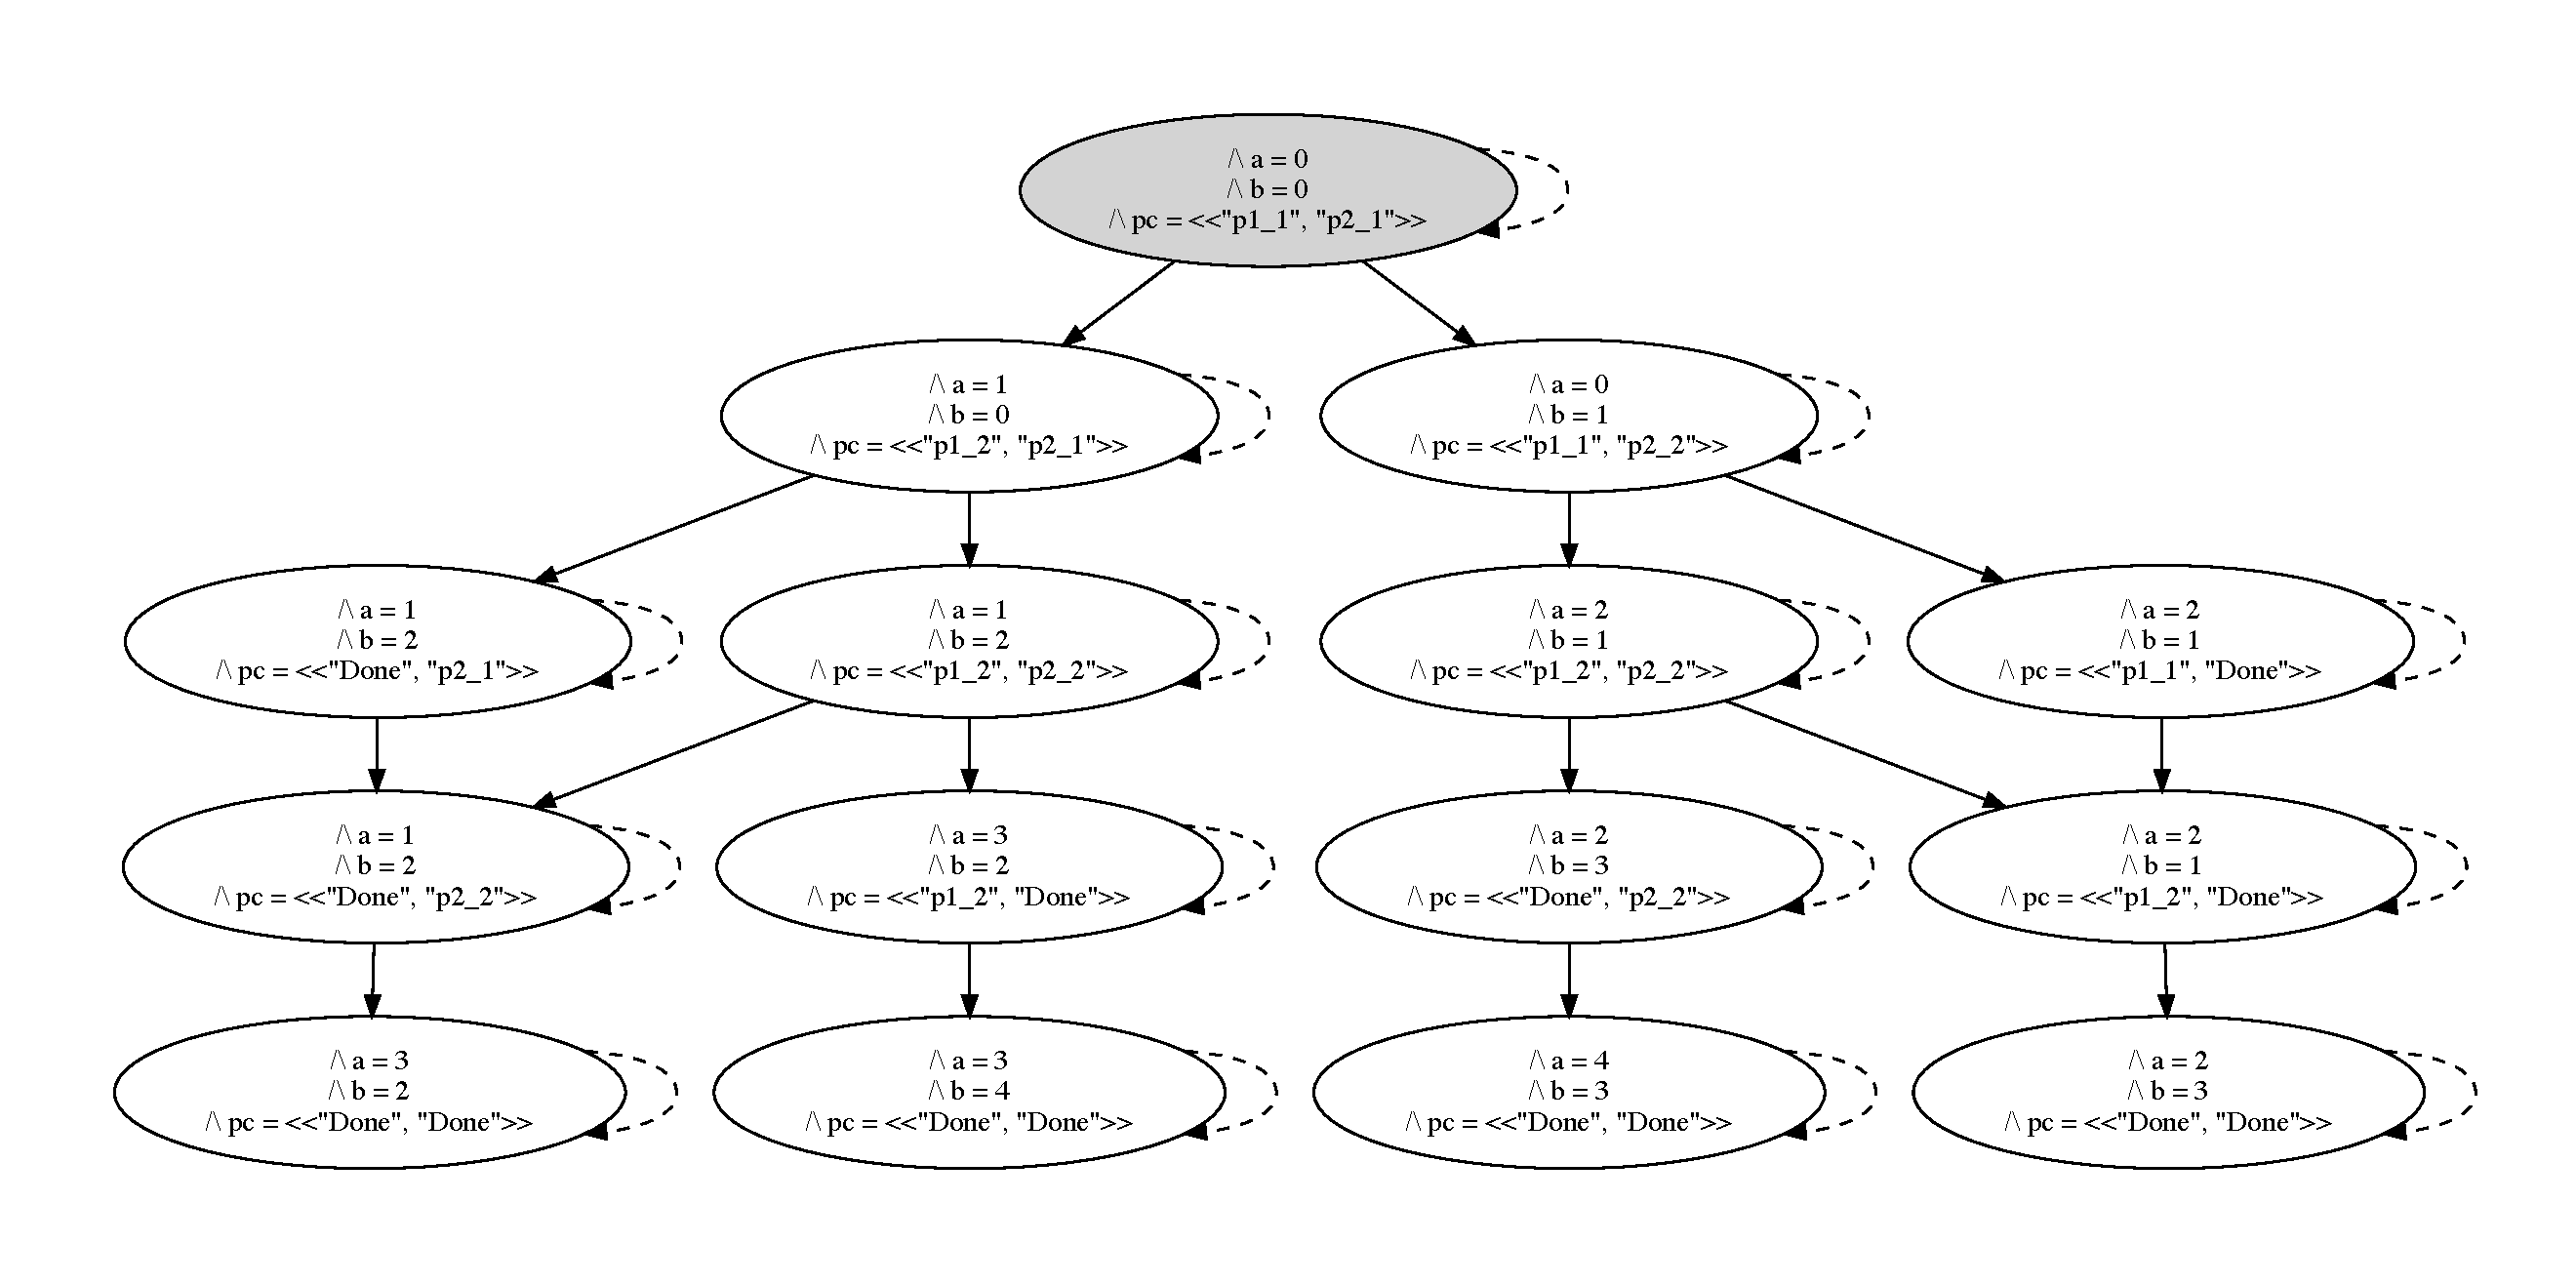
\includegraphics{02_PCDemo.pdf}};
    \draw[visible on=<2>,ultra thick,red,rounded corners] (12.2,1.5) rectangle (32.7,5.25);
  \end{tikzpicture}}%
\end{frame}

\begin{frame}[t,fragile]
  \frametitle{TLA+/PlusCal}
  \framesubtitle{Sets}
  \only<+>{\setminted{highlightlines={1}}}%
  \only<+>{\setminted{highlightlines={2}}}%
  \only<+>{\setminted{highlightlines={3}}}%
  \only<+>{\setminted{highlightlines={4}}}%
  \only<+>{\setminted{highlightlines={5}}}%
  \only<+>{\setminted{highlightlines={6}}}%
  \only<+>{\setminted{highlightlines={7,8}}}%
  \only<+>{\setminted{highlightlines={9}}}%
  \begin{code}{tla}
    Procs == {1, 5, 8}
    Ops == {"inc", "dec"}
    Vals == 1..MaxValue
    Cmd == Ops \union {"nop"}
    {1, 2, 3} \ {2} = {1, 3}
    {1, 2} \intersect {2, 3} = {2}
    var \in 1..10
    ASSUME Var \notin Procs
    1 \in Nat = TRUE
  \end{code}
\end{frame}

\begin{frame}[t,fragile]
  \frametitle{TLA+/PlusCal}
  \framesubtitle{Functions}
  \only<+>{\setminted{highlightlines={1}}}%
  \only<+>{\setminted{highlightlines={2}}}%
  \only<+>{\setminted{highlightlines={3}}}%
  \only<+>{\setminted{highlightlines={4,5}}}%
  \only<+>{\setminted{highlightlines={6,7}}}%
  \begin{code}{tla}
    Squares == [n \in Nat |-> n * n]
    Squares[2] = 4
    DOMAIN Squares = Nat
    F == [n \in 1..3 |-> n * n]
    DOMAIN F = 1..3
    Q == [F EXCEPT ![2] = 0]
    {Q[i]: i \in DOMAIN Q} = {1, 0, 9}
  \end{code}
\end{frame}

\begin{frame}[t,fragile]
  \frametitle{TLA+/PlusCal}
  \framesubtitle{Tuples}
  \only<+>{\setminted{highlightlines={1}}}%
  \only<+>{\setminted{highlightlines={2}}}%
  \only<+>{\setminted{highlightlines={3}}}%
  \only<+>{\setminted{highlightlines={4}}}%
  \only<+>{\setminted{highlightlines={5,6}}}%
  \only<+>{\setminted{highlightlines={7}}}%
  \only<+>{\setminted{highlightlines={8}}}%
  \only<+>{\setminted{highlightlines={9}}}%
  \only<+>{\setminted{highlightlines={10}}}%
  \only<+>{\setminted{highlightlines={11}}}%
  \begin{code}{tla}
    a == <<1, 5, 8>>
    DOMAIN a = 1..3
    a[2] = 5
    Len(a) = 3
    Head(a) = 1
    Tail(a) = <<5, 8>>
    SubSeq(a, 1, 2) = <<1, 5>>
    SelectSeq(a, LAMBDA i: i > 5) = <<8>>
    <<1, 2>> \o <<4, 8>> = <<1, 2, 4, 8>>
    a := Append(a, 5)
    a[i] := i
  \end{code}
\end{frame}

\begin{frame}[t,fragile]
  \frametitle{TLA+/PlusCal}
  \framesubtitle{Records}
  \only<+>{\setminted{highlightlines={1}}}%
  \only<+>{\setminted{highlightlines={2}}}%
  \only<+>{\setminted{highlightlines={3,4}}}%
  \only<+>{\setminted{highlightlines={5}}}%
  \only<+>{\setminted{highlightlines={6}}}%
  \only<+>{\setminted{highlightlines={7}}}%
  \only<+>{\setminted{highlightlines={8}}}%
  \only<+>{\setminted{highlightlines={9}}}%
  \begin{code}{tla}
    s == [rdy|->0, ack|->0, val|->0]
    DOMAIN s = {"rdy", "ack", "val"}
    s.rdy = 0
    s["ack"] = 0
    "a" :> 1 = [a|->1]
    [a->1] @@ [b|->2] = [a|->1, b|->2]
    [s EXCEPT !.rdy = @ + 1] = [rdy->1, ack|->0, val|->0]
    s.ack := 1
    [i \in DOMAIN s \ {"ack"} |-> s[i]] = [rdy|->0, val|->0]
  \end{code}
\end{frame}

\def\lh{\ttfamily\fontsize{11}{11}\selectfont}

\begin{frame}[c,fragile]
  \frametitle{Задача}
  \begin{center}
    \centering
    \begin{tikzpicture}[font=\sffamily]
      \tikzstyle{centrex}=[
        draw, thick, fill=yellow!20,
        text centered,
        minimum height=1.5em,
        drop shadow
      ]
      \tikzstyle{history}=[
        draw, thick, fill=green!20,
        text centered,
        minimum height=1.5em,
        drop shadow
      ]
      \tikzstyle{connection}=[
        red!60!black, draw, thick, -stealth
      ]
      \tikzstyle{connection text}=[
        black!80, midway, sloped, font=\ttfamily
      ]
      \node (fe1) [centrex] {Centrex Node};
      \node (fe2) [centrex, below=0.25cm of fe1] {Centrex Node};
      \path let \p1=(fe1.south east), \p2=(fe2.north east) in
         node (fe) at ($(\p1)!0.5!(\p2)$) {};
      \node (q) [history, right=1cm of fe] {Queue};
      \node (p) [history, right=1cm of q] {Processor};
      \node (db) [history, right=1cm of p] {Store};
      \path [connection] (fe1.east) -- (q) node [connection text, above] {\tiny CDR};
      \path [connection] (fe2.east) -- (q) node [connection text, below] {\tiny CDR};
      \path [connection] (q) -- (p);
      \path [connection] (p) -- (db);
    \end{tikzpicture}
  \end{center}
\end{frame}

\begin{frame}[c]
  \centering\Large\bf
  Модель:\\требования
\end{frame}

% v0
\begin{frame}[t,fragile]
  \frametitle{\lh CallHistory.tla v0}
  \only<+>{\setminted{highlightlines={5}}}%
  \only<+>{\setminted{highlightlines={10-11}}}%
  \only<+>{\setminted{highlightlines={14-17}}}%
  \only<+>{\setminted{highlightlines={19}}}%
  \only<+>{\setminted{highlightlines={23-26}}}%
  \only<+>{\setminted{highlightlines={28-34}}}%
  \only<+>{\setminted{highlightlines={30-33}}}%
  \begin{minipage}{\textwidth}
    \begin{columns}[T]
      \begin{column}{.45\textwidth}
        \inputtla[firstline=1,lastline=22]{example/v00/CallHistory.tla}
      \end{column}
      \begin{column}{.45\textwidth}
        \inputtla[firstline=23,lastline=36]{example/v00/CallHistory.tla}
      \end{column}
    \end{columns}
  \end{minipage}
\end{frame}

\begin{frame}[t,fragile]
  \frametitle{\lh CallHistory.cfg v0}
  \only<+>{\setminted{highlightlines={4,5}}}%
  \only<+>{\setminted{highlightlines={7,8}}}%
  \inputcode[firstline=1,lastline=8]{text}{example/v00/CallHistory.cfg}
\end{frame}

\begin{frame}[t,fragile]
  \frametitle{\lh CallHistory.tla v0 Run: {\color{red!80!black} Failed}}
  \only<+>{\setminted{highlightlines={21}}}%
  \only<+>{\setminted{highlightlines={23,65}}}%
  \only<+>{\setminted{highlightlines={67-70}}}%
  \only<+>{\setminted{highlightlines={73}}}%
  \only<+>{\setminted{highlightlines={75-76}}}%
  \inputcode[firstline=19,lastline=23]{text}{example/v00/modelling-result.txt}
  \inputcode[firstline=64,lastline=76]{text}{example/v00/modelling-result.txt}
\end{frame}

\begin{frame}[c]
  \centering\Large\bf
  Модель:\\первая реализация
\end{frame}

% v1
\begin{frame}[t,fragile]
  \frametitle{\lh CallHistory.tla v0->v1}
  \only<+>{\setminted{highlightlines={35}}}%
  \only<+>{\setminted{highlightlines={37}}}%
  \inputdiff[firstline=15,lastline=16]{example/v01/increment.diff}%
  \inputdiff[firstline=32,lastline=39]{example/v01/increment.diff}%
\end{frame}

\begin{frame}[t,fragile]
  \frametitle{\lh CallHistory.tla v0->v1}
  \only<+>{\setminted{highlightlines={19}}}%
  \only<+>{\setminted{highlightlines={12}}}%
  \only<+>{\setminted{highlightlines={13}}}%
  \inputdiff[firstline=10,lastline=30]{example/v01/increment.diff}%
\end{frame}

\begin{frame}[t,fragile]
  \frametitle{\lh CallHistory.tla v0->v1}
  \only<+>{\setminted{highlightlines={42}}}%
  \only<+>{\setminted{highlightlines={43}}}%
  \only<+>{\setminted{highlightlines={46}}}%
  \only<+>{\setminted{highlightlines={49}}}%
  \only<+>{\setminted{highlightlines={51}}}%
  \only<+>{\setminted{highlightlines={52}}}%
  \only<+>{\setminted{highlightlines={53}}}%
  \only<+>{\setminted{highlightlines={54}}}%
  \only<+>{\setminted{highlightlines={55}}}%
  \only<+>{\setminted{highlightlines={58}}}%
  \only<+>{\setminted{highlightlines={59}}}%
  \inputdiff[firstline=40,lastline=61]{example/v01/increment.diff}%
\end{frame}

\begin{frame}[t,fragile]
  \frametitle{\lh CallHistory.tla v1 Run: {\color{green!60!black} Succeed}}
  \only<+>{\setminted{highlightlines={22}}}%
  \only<+>{\setminted{highlightlines={26}}}%
  \inputcode[firstline=22,lastline=28]{text}{example/v01/modelling-result.txt}
\end{frame}

\begin{frame}[c]
  \centering\Large\bf
  Модель:\\добавим graceful shutdown
\end{frame}

% v2
\begin{frame}[t,fragile]
  \frametitle{\lh CallHistory.tla v1->v2}
  \only<+>{\setminted{highlightlines={20}}}%
  \only<+>{\setminted{highlightlines={40-44}}}%
  \only<+>{\setminted{highlightlines={42}}}%
  \only<+>{\setminted{highlightlines={43}}}%
  \inputdiff[firstline=15,lastline=21]{example/v02/increment.diff}%
  \inputdiff[firstline=32,lastline=44]{example/v02/increment.diff}%
\end{frame}

\begin{frame}[t,fragile]
  \frametitle{\lh CallHistory.tla v1->v2}
  \only<+>{\setminted{highlightlines={52,66,69}}}%
  \only<+>{\setminted{highlightlines={67,68}}}%
  \inputdiff[firstline=50,lastline=71]{example/v02/increment.diff}
\end{frame}

\begin{frame}[t,fragile]
  \frametitle{\lh CallHistory.tla v1->v2}
  \only<+>{\setminted{highlightlines={9}}}%
  \inputcode[firstline=1,lastline=9]{text}{example/v02/CallHistory.cfg}
\end{frame}

\begin{frame}[t,fragile]
  \frametitle{\lh CallHistory.tla v2 Run: {\color{red!80!black} Failed}}
  \only<+>{\setminted{highlightlines={23, 307}}}%
  \only<+>{\setminted{highlightlines={310-314}}}%
  \only<+>{\setminted{highlightlines={308, 315, 323}}}%
  \only<+>{\setminted{highlightlines={309}}}%
  \inputcode[firstline=21,lastline=23]{text}{example/v02/modelling-result.txt}
  \inputcode[firstline=306,lastline=323]{text}{example/v02/modelling-result.txt}
\end{frame}

% v3
\begin{frame}[t,fragile]
  \frametitle{\lh CallHistory.tla v2->v3}
  \only<+>{\setminted{highlightlines={68}}}%
  \inputdiff[firstline=50,lastline=71]{example/v03/increment.diff}%
\end{frame}

\begin{frame}[t,fragile]
  \frametitle{\lh CallHistory.tla v3 Run: {\color{red!80!black} Failed}}
  \only<+>{\setminted{highlightlines={23, 149}}}%
  \only<+>{\setminted{highlightlines={151}}}%
  \only<+>{\setminted{highlightlines={150}}}%
  \only<+>{\setminted{highlightlines={165,157}}}%
  \inputcode[firstline=21,lastline=24]{text}{example/v03/modelling-result.txt}
  \inputcode[firstline=148,lastline=165]{text}{example/v03/modelling-result.txt}
\end{frame}

% v4
\begin{frame}[t,fragile]
  \frametitle{\lh CallHistory.tla v3->v4}
  \only<+>{\setminted{highlightlines={68}}}%
  \inputdiff[firstline=54,lastline=72]{example/v04/increment.diff}%
\end{frame}

\begin{frame}[t,fragile]
  \frametitle{\lh CallHistory.tla v4 Run: {\color{green!60!black} Succeed}}
  \only<+>{\setminted{highlightlines={22}}}%
  \only<+>{\setminted{highlightlines={26}}}%
  \inputcode[firstline=22,lastline=27]{text}{example/v04/modelling-result.txt}
\end{frame}

\begin{frame}[c]
  \centering\Large\bf
  Модель:\\добавим аварийный останов
\end{frame}

% v5
\begin{frame}[t,fragile]
  \frametitle{\lh CallHistory.tla v4->v5}
  \only<+>{\setminted{highlightlines={75,76}}}%
  \only<+>{\setminted{highlightlines={50,72,74}}}%
  \inputdiff[firstline=47,lastline=56]{example/v05/increment.diff}%
  \vskip1ex%
  \inputdiff[firstline=71,lastline=76]{example/v05/increment.diff}%
\end{frame}

\begin{frame}[t,fragile]
  \frametitle{\lh CallHistory.tla v4->v5}
  \only<+>{\setminted{highlightlines={6}}}%
  \inputcode[firstline=1,lastline=11]{text}{example/v05/CallHistory.cfg}
\end{frame}

\begin{frame}[t,fragile]
  \frametitle{\lh CallHistory.tla v5 Run: {\color{red!80!black} Failed}}
  \only<+>{\setminted{highlightlines={23,406}}}%
  \only<+>{\setminted{highlightlines={408}}}%
  \only<+>{\setminted{highlightlines={410-414}}}%
  \only<+>{\setminted{highlightlines={415,423}}}%
  \only<+>{\setminted{highlightlines={407}}}%
  \inputcode[firstline=21,lastline=23]{text}{example/v05/modelling-result.txt}
  \inputcode[firstline=405,lastline=425]{text}{example/v05/modelling-result.txt}
\end{frame}

\begin{frame}[t,fragile]
  \frametitle{\lh CallHistory.tla v5 Run: {\color{red!80!black} Failed}}
  \only<+>{\setminted{highlightlines={150}}}%
  \only<+>{\setminted{highlightlines={144}}}%
  \only<+>{\setminted{highlightlines={151,154,158}}}%
  \inputcode[firstline=142,lastline=158]{text}{example/v05/modelling-result.txt}
\end{frame}

\begin{frame}[t,fragile]
  \frametitle{\lh CallHistory.tla v5 Run: {\color{red!80!black} Failed}}
  \setminted{highlightlines={162}}%
  \inputcode[firstline=160,lastline=176]{text}{example/v05/modelling-result.txt}
\end{frame}

% v6

\begin{frame}[t,fragile]
  \frametitle{\lh CallHistory.tla v5->v6}
  \only<+>{\setminted{highlightlines={61}}}%
  \only<+>{\setminted{highlightlines={74,14}}}%
  \only<+>{\setminted{highlightlines={76,80}}}%
  \inputdiff[firstline=13,lastline=13]{example/v06/increment.diff}%
  \vskip1ex%
  \inputdiff[firstline=58,lastline=80]{example/v06/increment.diff}%
\end{frame}

\begin{frame}[t,fragile]
  \frametitle{\lh CallHistory.tla v5->v6}
  \only<+>{\setminted{highlightlines={89}}}%
  \inputdiff[firstline=81,lastline=94]{example/v06/increment.diff}%
\end{frame}

\begin{frame}[t,fragile]
  \frametitle{\lh CallHistory.tla v5->v6}
  \inputdiff[firstline=24,lastline=28]{example/v06/increment.diff}%
  \pause%
  \only<+>{\setminted{highlightlines={30}}}%
  \only<+>{\setminted{highlightlines={31}}}%
  \only<+>{\setminted{highlightlines={32}}}%
  \only<+>{\setminted{highlightlines={33}}}%
  \only<+>{\setminted{highlightlines={34}}}%
  \inputdiff[firstline=29,lastline=43]{example/v06/increment.diff}%
\end{frame}

\begin{frame}[t,fragile]
  \frametitle{\lh CallHistory.tla v6 Run: {\color{red!80!black} Failed}}
  \only<+>{\setminted{highlightlines={23,543}}}%
  \only<+>{\setminted{highlightlines={545}}}%
  \only<+>{\setminted{highlightlines={544}}}%
  \inputcode[firstline=23,lastline=23]{text}{example/v06/modelling-result.txt}
  \inputcode[firstline=542,lastline=563]{text}{example/v06/modelling-result.txt}
\end{frame}

% v7
\begin{frame}[t,fragile]
  \frametitle{\lh CallHistory.tla v6->v7}
  \only<+>{\setminted{highlightlines={24}}}%
  \only<+>{\setminted{highlightlines={80}}}%
  \only<+>{\setminted{highlightlines={41}}}%
  \inputdiff[firstline=19,lastline=24]{example/v07/increment.diff}%
  \vskip1ex%
  \inputdiff[firstline=36,lastline=42]{example/v07/increment.diff}%
  \vskip1ex%
  \inputdiff[firstline=75,lastline=81]{example/v07/increment.diff}%
\end{frame}

\begin{frame}[t,fragile]
  \frametitle{\lh CallHistory.tla v7 Run: {\color{green!60!black} Succeed}}
  \only<+>{\setminted{highlightlines={22}}}%
  \only<+>{\setminted{highlightlines={26}}}%
  \inputcode[firstline=22,lastline=27]{text}{example/v07/modelling-result.txt}
\end{frame}

\begin{frame}[c]
  \centering\Large\bf
  Модель:\\добавим аварийный сброс вызова
\end{frame}

% v8
\begin{frame}[t,fragile]
  \frametitle{\lh CallHistory.tla v7->v8}
  \only<+>{\setminted{highlightlines={46,48,50}}}%
  \only<+>{\setminted{highlightlines={49}}}%
  \inputdiff[firstline=42,lastline=51]{example/v08/increment.diff}%
\end{frame}

\begin{frame}[t,fragile]
  \frametitle{\lh CallHistory.tla v8 Run: {\color{red!80!black} Failed}}
  \only<+>{\setminted{highlightlines={23,357}}}%
  \only<+>{\setminted{highlightlines={359}}}%
  \only<+>{\setminted{highlightlines={358}}}%
  \inputcode[firstline=21,lastline=23]{text}{example/v08/modelling-result.txt}
  \inputcode[firstline=356,lastline=376]{text}{example/v08/modelling-result.txt}
\end{frame}

% v9
\begin{frame}[t,fragile]
  \frametitle{\lh CallHistory.tla v8->v9}
  \only<+>{\setminted{highlightlines={23}}}%
  \only<+>{\setminted{highlightlines={38}}}%
  \only<+>{\setminted{highlightlines={52}}}%
  \inputdiff[firstline=19,lastline=24]{example/v09/increment.diff}%
  \vskip1ex%
  \inputdiff[firstline=37,lastline=40]{example/v09/increment.diff}%
  \vskip1ex%
  \inputdiff[firstline=44,lastline=54]{example/v09/increment.diff}%
  \vskip1ex%
\end{frame}

\begin{frame}[t,fragile]
  \frametitle{\lh CallHistory.tla v9 Run: {\color{red!80!black} Failed}}
  \only<+>{\setminted{highlightlines={23,318}}}%
  \only<+>{\setminted{highlightlines={335,319}}}%
  \only<+>{\setminted{highlightlines={320,321}}}%
  \inputcode[firstline=21,lastline=23]{text}{example/v09/modelling-result.txt}
  \inputcode[firstline=317,lastline=337]{text}{example/v09/modelling-result.txt}
\end{frame}

% v10
\begin{frame}[t,fragile]
  \frametitle{\lh CallHistory.tla v9->v10}
  \only<+>{\setminted{highlightlines={67}}}%
  \only<+>{\setminted{highlightlines={71}}}%
  \only<+>{\setminted{highlightlines={79}}}%
  \only<+>{\setminted{highlightlines={12}}}%
  \inputdiff[firstline=10,lastline=12]{example/v10/increment.diff}%
  \vskip1ex%
  \inputdiff[firstline=62,lastline=80]{example/v10/increment.diff}%
\end{frame}

\begin{frame}[t,fragile]
  \frametitle{\lh CallHistory.tla v9->v10}
  \only<+>{\setminted{highlightlines={92}}}%
  \only<+>{\setminted{highlightlines={95}}}%
  \only<+>{\setminted{highlightlines={96}}}%
  \only<+>{\setminted{highlightlines={98}}}%
  \only<+>{\setminted{highlightlines={99}}}%
  \only<+>{\setminted{highlightlines={100}}}%
  \only<+>{\setminted{highlightlines={52,101}}}%
  \inputdiff[firstline=47,lastline=53]{example/v10/increment.diff}%
  \vskip1ex%
  \inputdiff[firstline=88,lastline=103]{example/v10/increment.diff}%
\end{frame}

\begin{frame}[t,fragile]
  \frametitle{\lh CallHistory.tla v9->v10}
  \only<+>{\setminted{highlightlines={7}}}%
  \inputcode[firstline=1,lastline=11]{text}{example/v10/CallHistory.cfg}
\end{frame}

\begin{frame}[t,fragile]
  \frametitle{\lh CallHistory.tla v10 Run: {\color{red!80!black} Failed}}
  \only<+>{\setminted{highlightlines={23,532}}}%
  \only<+>{\setminted{highlightlines={542,536}}}%
  \only<+>{\setminted{highlightlines={553}}}%
  \inputcode[firstline=23,lastline=23]{text}{example/v10/modelling-result.txt}
  \inputcode[firstline=531,lastline=553]{text}{example/v10/modelling-result.txt}
\end{frame}

% v11
\begin{frame}[t,fragile]
  \frametitle{\lh CallHistory.tla v10->v11}
  \only<+>{\setminted{highlightlines={90}}}%
  \only<+>{\setminted{highlightlines={91}}}%
  \only<+>{\setminted{highlightlines={92,93}}}%
  \inputdiff[firstline=86,lastline=95]{example/v11/increment.diff}%
\end{frame}

\begin{frame}[t,fragile]
  \frametitle{\lh CallHistory.tla v11 Run: {\color{green!60!black} Succeed}}
  \only<+>{\setminted{highlightlines={25}}}%
  \only<+>{\setminted{highlightlines={30}}}%
  \only<+>{\setminted{highlightlines={31}}}%
  \inputcode[firstline=25,lastline=31]{text}{example/v11/modelling-result.txt}
\end{frame}

\begin{frame}[c]
  \centering\Large\bf
  Модель:\\итог
\end{frame}

\begin{frame}[t,fragile]
  \frametitle{\lh CallHistory.tla v11}
  \inputtla[firstline=1,lastline=24]{example/v11/CallHistory.tla}
\end{frame}

\begin{frame}[t,fragile]
  \frametitle{\lh CallHistory.tla v11}
  \inputtla[firstline=25,lastline=48]{example/v11/CallHistory.tla}
\end{frame}

\begin{frame}[t,fragile]
  \frametitle{\lh CallHistory.tla v11}
  \inputtla[firstline=49,lastline=72]{example/v11/CallHistory.tla}
\end{frame}

\begin{frame}[t,fragile]
  \frametitle{\lh CallHistory.tla v11}
  \inputtla[firstline=73,lastline=96]{example/v11/CallHistory.tla}
\end{frame}

\begin{frame}[t,fragile]
  \frametitle{\lh CallHistory.tla v11}
  \inputtla[firstline=97,lastline=113]{example/v11/CallHistory.tla}
\end{frame}

% Продолжение

\begin{frame}[c, fragile]
  \begin{center}
    \centering
    \includegraphics[keepaspectratio, height=.7\textheight]{in-and-out-final.jp2}\\%
    \fontsize{8}{8}\selectfont\color{white!70!black}\copyright The Cartoon Network%
  \end{center}
\end{frame}

\begin{frame}
  \centering\Large\bf{С чего начать?}
\end{frame}

\begin{frame}[c]
  \begin{columns}
    \begin{column}{.47\textwidth}
      \begin{minipage}[c][0.75\textheight][c]{\columnwidth}
        \centering%
        \href{https://www.apress.com/gp/book/9781484238288}{%
          
\includegraphics[keepaspectratio, height=.85\textheight]{practical-tla-cover.pdf}
        }%
      \end{minipage}%
    \end{column}
    \begin{column}{.47\textwidth}%
      \begin{minipage}[c][0.75\textheight][s]{\columnwidth}
        \href{https://www.apress.com/gp/book/9781484238288}{%
        {\Large\bf Practical \TLA}\\
        {\large\bf Planning Driven Development}\\%
        \\%
        {\normalsize by Hillel Wayne\\Apress, 2018}
      }\\%
      \\%
      {\large Только про PlusCal,\\%
      идеально для вхождения в тему!}\\%
      \vfill%
      \href{https://www.apress.com/gp/book/9781484238288}{%
        \qrcode[hyperlink,height=.2\textheight]{https://www.apress.com/gp/book/9781484238288}
      }
    \end{minipage}
    \end{column}
  \end{columns}
\end{frame}

\begin{frame}[c]
  \begin{columns}
    \begin{column}{.47\textwidth}
      \begin{minipage}[c][0.75\textheight][c]{\columnwidth}
      \centering%
      \href{https://lamport.azurewebsites.net/tla/book.html\#download}{%
        
\includegraphics[keepaspectratio, height=.85\textheight]{specifying-systems-cover.jpg}
      }%
      \end{minipage}%
    \end{column}
    \begin{column}{.47\textwidth}
      \begin{minipage}[c][0.75\textheight][s]{\columnwidth}
      \href{https://lamport.azurewebsites.net/tla/book.html\#download}{%
        {\Large\bf Specifying Systems}\\%
        {\large\bf The \TLA\ Language and Tools\\%
        for Hardware and Software\\%
        Engineers}\\%
        {\normalsize by Leslie Lamport\\Addison-Wesley Professional, 2002}%
      }%
      \\%
      \\%
      {\large \TLA, обязательно иметь под рукой}%
      \vfill%
      \href{https://lamport.azurewebsites.net/tla/book.html\#download}{%
         \qrcode[hyperlink,height=.2\textheight]{https://lamport.azurewebsites.net/tla/book.html\#download}
      }%
      \end{minipage}%
    \end{column}
  \end{columns}
\end{frame}

\begin{frame}[c]
  \begin{columns}
    \begin{column}{.47\textwidth}
      \begin{minipage}[c][0.75\textheight][c]{\columnwidth}
      \centering%
      \href{http://lamport.azurewebsites.net/video/videos.html}{%
        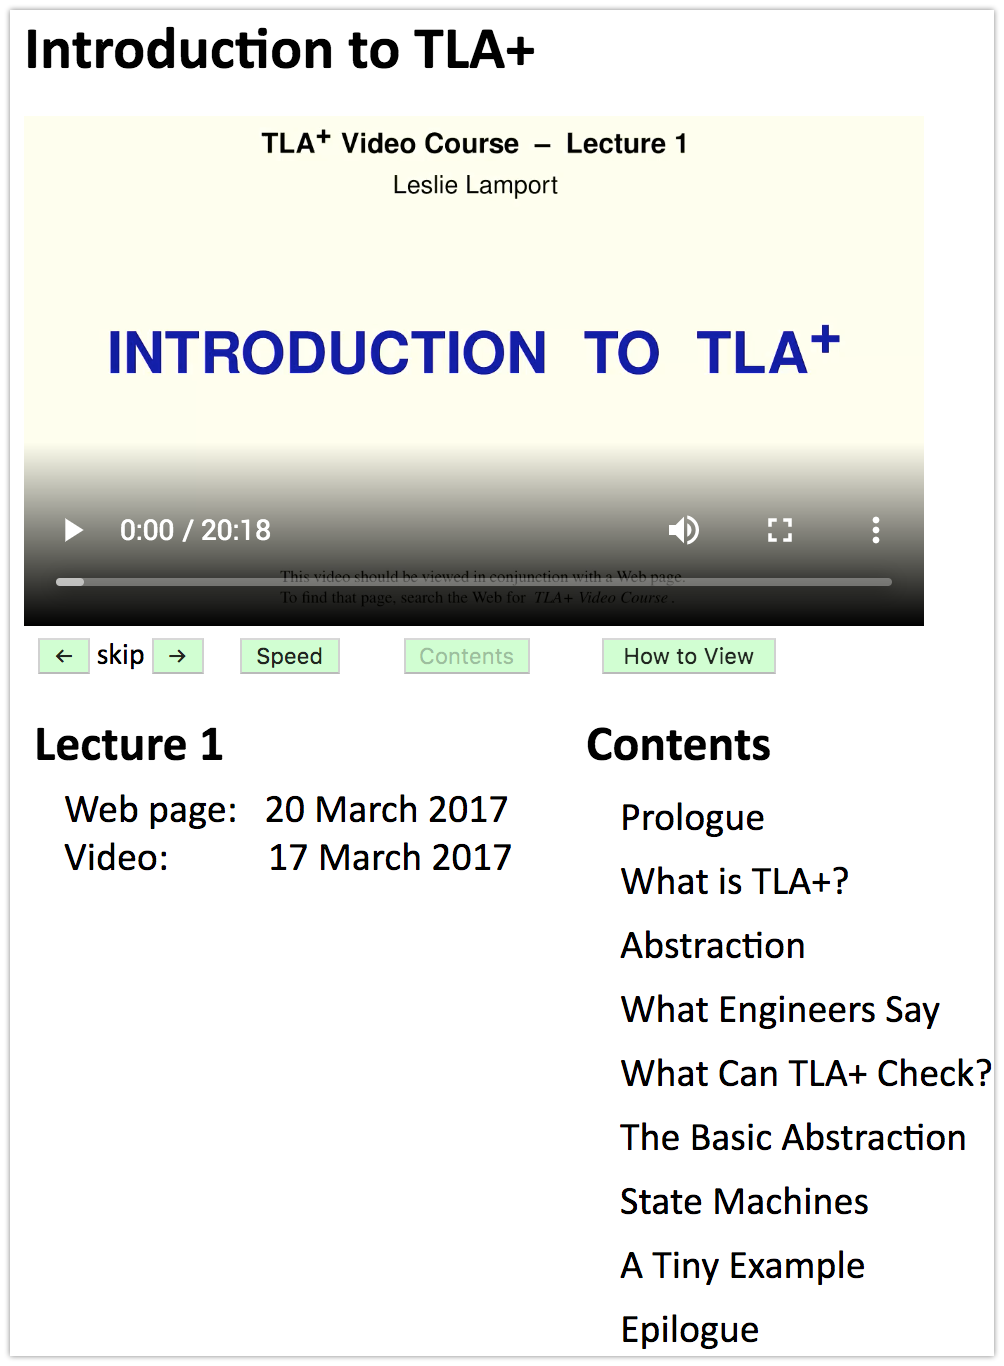
\includegraphics[keepaspectratio, height=.85\textheight]{tla-video-course-cover.png}
      }%
      \end{minipage}%
    \end{column}
    \begin{column}{.47\textwidth}
      \begin{minipage}[c][0.75\textheight][s]{\columnwidth}
      \href{http://lamport.azurewebsites.net/video/videos.html}{%
        {\Large\bf \TLA\ Video Course}\\
        {\normalsize by Leslie Lamport}
      }\\
      \\
      \large%
      3.5 часа \TLA,\\
      \\%
      \underline{обязательно} посмотреть!\\
      \\%
      (Лэмпорт прекрасный лектор!)\\
      \vfill
      \href{http://lamport.azurewebsites.net/video/videos.html}{%
        \qrcode[hyperlink,height=.2\textheight]{http://lamport.azurewebsites.net/video/videos.html}
      }
      \end{minipage}
    \end{column}
  \end{columns}
\end{frame}

\begin{frame}[c]
  \centering\large%
  \vfill%
  \begin{beamercolorbox}{}
    Lamport \TLA\ Site: \href{https://lamport.azurewebsites.net/tla/tla.html}{\textcolor{blue}{https://lamport.azurewebsites.net/tla/tla.html}}\\[2ex]
    Learn \TLA: \href{https://learntla.com/}{\textcolor{blue}{https://learntla.com}}\\[2ex]
    google group: \href{https://groups.google.com/forum/\#!forum/tlaplus}{\textcolor{blue}{https://groups.google.com/forum/\#!forum/tlaplus}}\\[2ex]
    reddit: \href{https://www.reddit.com/r/tlaplus/}{\textcolor{blue}{https://www.reddit.com/r/tlaplus/}}\\[2ex]
    \TLA\ Tools: \href{https://github.com/tlaplus/tlaplus}{\textcolor{blue}{https://github.com/tlaplus/tlaplus}}
  \end{beamercolorbox}
  \vfill%
\end{frame}

\begin{frame}[t]
  \frametitle{Q\&A}
  \begin{itemize}
    \item \TLA\ -- это недели проектирования и месяцы кодирования?
    \begin{itemize}
      \item Нет, это часы моделирования и дни или недели работы.
    \end{itemize}
    \item Что насчет COQ (Agda, Idris, ...)?
    \begin{itemize}
      \item Принципиально разная сложность
      \item (есть еще \href{https://github.com/informalsystems/apalache}{Apalache ({\ttfamily github.com/informalsystems/apalache})} by \href{https://informal.systems/}{Informal Systems})
    \end{itemize}
    \item Что насчет Alloy?
    \begin{itemize}
      \item Тоже отличный выбор для инженерных задач
    \end{itemize}
    \item Можно ли из спецификации сразу делать код?
    \begin{itemize}
      \item Можно, но не нужно (см. \href{https://github.com/UBC-NSS/pgo}{PGo ({\ttfamily github.com/UBC-NSS/pgo})})
      \item (но если очень нужно, то есть Agda и Idris)
    \end{itemize}
  \end{itemize}
\end{frame}

\newcommand{\btVFill}{\vskip0pt plus 1filll}
\begin{frame}
  \centering%
  \btVFill%
  {\Huge\bf Спасибо!}
  \btVFill%
\end{frame}

\end{document}
%%% Local Variables:
%%% mode: latex
%%% TeX-master: t
%%% End:
